\PassOptionsToPackage{greek,english}{babel}
\documentclass{NSF_proposal_mod}

%PI: vardavas
%NSF ID: 000580367
%password:RedJupiter5
%Temp. Proposal #7091864
% Pin: 1234

% Pages to split the pdf at. 1,2,17,25,28,29,30



%\usepackage{epsfig}
%\documentclass[11pt]{article}

\usepackage[numbers,sort&compress]{natbib}


\usepackage[dvips]{graphicx}
\usepackage[table]{xcolor}
\usepackage{setspace}
\usepackage{enumitem}
\usepackage{adjustbox}
\usepackage{color}
\usepackage{boxedminipage}
\usepackage{amsfonts}
\usepackage{amsmath}
\usepackage{url}
\usepackage{caption}
\usepackage{tikz}
%\usepackage{setspace}
\usepackage{hyperref}
\usepackage{wrapfig}
\usepackage[T1]{fontenc}
\usepackage{tablefootnote}
\usepackage{multirow}
\usepackage{float} %After doing some more googling I came across the float package 
\restylefloat{table} %which lets you prevent LaTeX from repositioning the tables.
\usepackage[inline]{trackchanges} 
%\usepackage[margins]{trackchanges}
\addeditor{rv}
\addeditor{ap} 
\addeditor{kb} 
\addeditor{rl}
\addeditor{kk}
\addeditor{ga}
%%% Greek language
\usepackage[iso-8859-7]{inputenc}


%%% These lines of code deal with breaking up long url links.
\makeatletter
\g@addto@macro{\UrlBreaks}{\UrlOrds}
\makeatother

% NSF proposal generation template style file.
% based on latex stylefiles  written by Stefan Llewellyn Smith and
% Sarah Gille, with contributions from other collaborators.

\newcommand{\jas}{{\it J. Atmos. Sci.}}
\newcommand{\jpo}{{\it J. Phys. Oceanogr.}}
\newcommand{\JPO}{{\it J. Phys. Oceanogr.}}
\newcommand{\jfm}{{\it J. Fluid Mech.}}
\newcommand{\jgr}{{\it J. Geophys. Res.}}
\newcommand{\JGR}{{\it J. Geophys. Res.}}
\newcommand{\jmr}{{\it J. Mar. Res.}}
\newcommand{\arfm}{{\it Ann. Rev. Fluid Mech.}}
\newcommand{\dsr}{{\it Deep-Sea Res.}}
\newcommand{\dao}{{\it Dyn. Atmos. Oceans}}
\newcommand{\jam}{{\it Journal of Applied Meteorology}}
\newcommand{\phfl}{{\it Phys. Fluids}}
\newcommand{\phfla}{{\it Phys. Fluids A}}
\newcommand{\PhilTrans}{{\it Philosophical Transactions of the Royal Society, 
London}}
\newcommand{\gafd}{{\it Geophys. Astrophys. Fluid Dyn.}}
\newcommand{\gfd}{{\it Geophys. Fluid Dyn.}}
\newcommand{\PCE}   {{\it Physics and Chemistry of the Earth}}
\newcommand{\PRL}   {{\it Physical Review Letters}}

\newcommand{\ProgOc}{{\it Prog. Oceanography}}
\newcommand{\WHOITR}{Woods Hole Oceanographic Institution Technical Report, WHOI-}
\newcommand{\degrees}{$\!\!$\char23$\!$}
\DeclareFontFamily{OT1}{psyr}{}
\DeclareFontShape{OT1}{psyr}{m}{n}{<-> psyr}{}
\def\times{{\fontfamily{psyr}\selectfont\char180}}

\definecolor{gold}{rgb}{0.85,.66,0}
\definecolor{QNblu}{rgb}{.33,.66,1}
\definecolor{QNblu2}{rgb}{.60,.40,.70}

\newcommand{\rv}[1]{\textbf{{\color{red} RV comment:}} \color{QNblu2}{ #1}}
\newcommand{\cut}[1] {\textbf{{\color{red} CUT }}  \color{gold}{ #1}}
\newcommand{\edit}[1] {\textbf{{\color{red} }}  \color{red}{ #1}}
\newcommand{\field}[1]{\mathbb{#1}}
\newcommand{\parnoind}{\ \\
\noindent}
\newcommand{\parnoindtwo}{\ \vspace{6pt} \\
\noindent}



\renewcommand{\refname}{\centerline{References cited}}

% this handles hanging indents for publications
\def\rrr#1\\{\par
\medskip\hbox{\vbox{\parindent=2em\hsize=6.12in
\hangindent=4em\hangafter=1#1}}}

\def\baselinestretch{1}

\begin{document}

\begin{center}
{\Large{\bf IBSS: An Agent-Based Model of the Role of \\ Income Tax Evasion Perceptions: Behavioral Model}}\\*[3mm]
%{\bf } \\*[3mm]
\end{center}
%\pagenumbering{arabic}
%\renewcommand{\thepage} {Title--\arabic{page}}

%\section*{Appendix B: Tables of Model Parameters}
%Below we present tables giving model parameters, their definition, whether we expect them to take different values depending on the population strata and the potential source for obtaining their ranges of values. Please note that this is a preliminary table and may not include all model parameters that will be used in the final model.  
%Our model considers three sets of model parameters: behavioral and economic parameters, social mixing parameters and influenza epidemiological parameters.  


% Add p.161 George Box; How will we Validate and Verify?; p.312 and 325 of Wilensky & Rand

%\pagenumbering{arabic}
%\renewcommand{\thepage} {Approach--\arabic{page}}

\section{General Framework of the Agent-Based Model}
\label{Sec:General}
%Here I describe the model as implemented in the prototype R code.


Our model considers $N$ individuals that every year make tax-related decisions. A fraction of these individuals have a type of employment (such as self-employment) that provides them with the opportunity to under-report their yearly income. These represent the population that can initiate in intentionally under-reporting their income.  Other individuals that have income from salaries always comply since their employer automatically withholds their income tax. We use $e$ to represent the self-employed share of total employment. Each individual $i$ is assigned an income $I^{(i)}$ sampled from an income distribution and on which they pay a fraction as taxes. We consider different tax brackets which depend on income. Here, for simplicity we describe the case for a single tax rate $T$. Revenues for tax collection are assumed to support public services however inevitably due to inefficiencies not all revenue is used to to support services. We assume that $v$ describes the per capita level of government services. 

\begin{wrapfigure}{r}{3.1in}%  figure placement: here, top, bottom, or page
\centering
\vspace{-20pt}
 \includegraphics[width=3in]{figures/Conceptual_Diagram.pdf} 
\vspace{-5pt}
   \label{Fig:ConceptualDiagram}
\caption{Conceptual Diagram showing individual decisions, outcomes and evaluations.}
\end{wrapfigure}
Individuals are connect in a social network whereby individual's can affect each others tax related perceptions.  Each individual $i$ has a fixed static set $\mathbf{J}^{(i)}$ of alters.  The model proceeds iteratively from year to year, respectively denoted by $t$ and $t+1$. The first step of this iteration stochastically selects the subset of alters of individual $i$ with whom s/he could be influenced $\mathbf{J}^{(i)}_t$ in year $t$.  Then individuals go through Decision-Outcome-Evaluation processes as illustrated by the conceptual diagram shown in figure \ref{Fig:ConceptualDiagram}. The first of these is the Decision process whereby individuals with an opportunity to under-report decide to either (i) comply in full, (ii) initiate in under-reporting, or (iii) continue to under-report their income. 
\vspace{5pt}

{\bf Decision:} Each individual $i$ has an associated endogenously determined proportion $w^{(i)}_t$ in year $t$ of their income they would like to report. Individuals with an opportunity to under-report that were compliant in the previous year stochastically initiate in tax-evasion with probability $1-w^{(i)}_t$. A similar rule applies to those individuals that were non-compliant in the previous year but were audited and penalized by the tax authority for under-reporting their taxes. Those that were non-compliant in the previous year which were not audited and penalized report the proportion $w^{(i)}_t$  of their income\footnote{ $w^{(i)}_t$  is smaller than 100\% for this population.}.

\note[kb]{I know we've talked about this before, but I still don't understand why $w_t^{(i)}$, which is the fraction of income individual i wants to report in time t, should influence the decision to initiate underreporting in the manner you specify. Using your suggested approach, if individual i wants to report 90 percent of their income but individual j wants to report just 10 percent of their income, then j is nine times more likely to initiate underreporting than i. Both want to underreport, perhaps with equal desire, it is just the fraction of income they want to report that varies between the two. I think you need to describe more clearly for the reader why it makes sense to use $w_t^{(i)}$ in this way. An alternative approach would be to base the likelihood of an individual to initiate underreporting on the mean fraction of the population of interest (i.e., self-employed) that underreports. For example, Figure 1 of Alm, Bloomquist, and McKee (2015) shows roughly 130 out of 1,101 randomly audited self-employed taxpayers (~ 12 percent) as being fully compliant. (Actually, 129 of the 1,101 taxpayers had a compliance rate of 100 percent or more, 133 taxpayers had a compliance rate of at least 99 percent, and 150 taxpayers had a compliance rate of 95 percent or higher. I can provide the raw data for all 1,101 taxpayers if you are interested.) Therefore, 88 percent of self-employed taxpayers underreport to some extent in any given year. }
\note[rv]{I agree that the amount that a (previously compliant) taxpayer wishes to underrepot expressed as a fraction of his income does not necessity relate directly to the probability s/he will act and initiate in evasion. So basically we can call the two concepts {\it propensity} to initiate in evasion and {\it intensity} of evasion on the year of initiation. The two are not necessarily related.  Although the relationship between propensity and intensity may not be as linear and direct as I have assumed here - it does seem to me very plausible that for the cases where the potential intensity is large, propensity is large too. The opposite may not generally be true - thus high propensity does not necessarily lead to high intensity. However, because of the former plausible link - when averaging over many cases - I think that we should see a weak but present correlation between the two.  

In this ABM - I would like to have behavioral mechanisms that are as endogenous to the model as possible. So my preference would be to calibrate the distributions for $c_1$ and the parameters that affect willingness to comply to produce distributions for $w_t^{(i)}$ that are in agreement with what is observed. Including your paper Alm, Bloomquist, and McKee (2015). This may be hard to do because not only do we need to get the parameters right but the behavioral model shouldn't too farfetched in a way that it makes the real world observations unattainable to be reproduced by the model. So I'm aware of this issue. Nevertheless, I would like to avoid the modeling the propensity to evade as a stochastic process that is in agreement with the observed data but doesn't depend on  an internal/endogenous evolutionary behavioral model based on the agents attributes.  However, during the process of our sensitivity analysis and calibration - I agree that we should be open to the possibility that the model will not calibrate well - and thus I may need to abandon such an idea. Thus - in preparation for that - I'll construct an alternative module that is based on data found in your paper with Alm, Bloomquist, and McKee (2015). {\bf Since you offered - it would indeed be great if we could get the raw data set to analyze - and use it at least for the calibration process. }Thanks!}


\note[kb]{I would further argue that although taxpayers who underreport would like to report only $w_t^{(i)}$ of their income, they may report more than $w_t^{(i)}$  (but less than 100 percent) due to uncertainty. Therefore, I recommend assuming a fixed probability of underreporting (for a previously compliant taxpayer) of 0.88 based on the data in Alm, Bloomquist, and McKee (2015) and then determine the fraction of income reported in time t, $(f_t)$ by generating a uniform random number $u~[0,1]$so that

$f_t=u$ when $u \le w_t^{(i)}$ and $f(t)= w_t^{(i)}$ otherwise  (1).

For noncompliant taxpayers not audited in the previous round, assume they will continue to be noncompliant but determine their new $f_t$ by generating a uniform random number $u~[0,f_(t-1)]$ and using equation (1) to determine the new $f_t$. Over time taxpayers that go unaudited will eventually settle on $w_t^{(i)}$ as their long-run reporting behavior.}
\note[rv]{This is a great point. I agree that taxpayers that initiate in underreporting will not under-report right way the full amount that they first wish to under-report based on fairness, detterance etc.,  but due to many other reasons (risk adversity, habit , views of self-esteem ) probably will begin slowly at first. Actually, this effect is captured in our model because fairness, detteranece, media, network interactions affect what I label as $\Delta_t^{(i)}$. In absence of any past experience $w_t^{(i)}=\Delta_t^{(i)}$. However, with past experience we get a {\it inertia effect} - whereby $w_t^{(i)}$ is determined by a weighted sum of $\Delta_t^{(i)}$. If a taxpayer was for many previous years compliant then $w_t^{(i)}>\Delta_t^{(i)}$, and thus if this taxpayer does stochastically (based on the behavioral model) initiate in underreporting, s/he will report more than $\Delta_t^{(i)}$ (i.e., $\Delta_t^{(i)}$ is his most recent feelings towards intensity of evasion). The opposite is true for taxpayers that have been under-reporting for many years. Their perceptions may change for various reasons (e.g.,  personal outcome, network effects, media and may have a $\Delta_t^{(i)}>w_t^{(i)}$. Relating to the specific equation (1) you list: I have a similar though not equivalent process described in equation \ref{eq:DeltaP}. Recall that $\Delta_t^{(i)}$ is made up by three components: personal, network and penalty feedbacks. The personal component is $\Delta_P^{(i)}$ and this can often be equal to 0 for taxpayers that are not compliant and successfully evade. Thus if $\Delta_P^{(i)}$ is always 0 , the self-employed taxpayer will eventually under-report all the income he can. However, $\Delta_P^{(i)}=0$ stochastically, and at times  $\Delta_P^{(i)}=w_t^{(i)}$, for non compliant taxpayers this leads to a process which over time leads to $w_t^{(i)} \to 0$ but often the under-reporting taxpayer may go through many years of reporting a fraction of their income before decaying to 0 as can be seen by the sample trajectory figures in fig. \ref{fig:trajectories1}.}

\note[rv]{See \cite{StevenE.Crane1990}  they state:  Our findings support the popular contention that evaders respond to higher marginal tax ratesby increasing their evasion activity. The results also confirm he theoretical predictionthat individuals with higher levels of income tend to evade more. }

{\bf Outcome:} Each individual can be audited by the tax authority. A fraction $q$ of the population, also known as the audit rate,  is selected for an audit every year. Individuals can be randomly or endogenously selected for an audit \footnote{Here endogenous auditing means that the tax authority uses a rule to target certain tax payers for an audit.}.  If caught evading, a penalty represented by a fraction $P$ of each year's tax underpayment is added to the total taxes due. Thus $P$ is also referred to as a penalty rate. We assume a maximum number of $K$ years of back-auditing that the tax authority may investigate an individual's tax records and apply penalties for any discovered evasion. Each individual $i$ has his/her own perceived audit and penalty rate respectively denoted by $\tilde{q}^{(i)}_t$ and $\tilde{P}^{(i)}_t$. As explained in detail in section \ref{Sec:Deterrance}, these perceptions change with personal experiences with tax audits and penalties for under-reporting. Moreover, $\tilde{q}^{(i)}_t$ can also be influenced by communication and observation with his/her alters  $\mathbf{J}^{(i)}_t$ and could be influenced by media.   

In our model, compliant individuals can have a refund return when they file their income taxes or be required to pay an additional amount of taxes. Whether s/he receives a refund return or is asked for further payment can also influence the taxpayer to initiate in tax evasion. We assume a simple Markov process, whereby compliant taxpayers can stochastically transition from a refund return to an addition payment state from year to year.      
 
The above represent individual-level outcomes. The model also considers aggregated macroscopic outcomes. Each individual is taxed at rate $T$ on their reported income given by $w^{(i)}_tI^{(i)}$. Summing these gives the total tax revenues. \remove[rv]{We further sum the total recovered revenues obtained by detected under-reporting of the tax payers by the tax audits as well as the totally amount received as penalties.} The difference between the expected revenues by the tax authority and this total sum, expressed as a fraction of the former gives the tax gap expressed as a proportion\footnote{For simplicity we assume that the expected revenue by the authorities is given by the sum of the $TI^{(i)}$ over all individuals.}.  As explained in detail in section \ref{Sec:Evaluations}, we assume that the media reports this information to the public with an overall frequency and intensity that depends on tax gap proportion.       

\note[kb]{Just to be clear, the definition of the 'tax gap' excludes penalties (and interest). The tax gap (expressed as a ratio) is: (tax reported) / (tax reported + net underreported tax). Note that under this definition the tax gap ratio can be > 1.}
\note[rv]{I'm a little confused about this. The definition I find online is {\it The difference between total amounts of taxes owed to the government versus the amount they actually receive.}. Based on this the expected revenues is (tax reported + net underreported tax) and the actual revenues is simply tax reported. This difference between the expected and the actual expressed as a proportion of the expected is (net underreported tax) / (tax reported + net underreported tax). I believe that is what you intended? Anyhow - based on your comment - I have removed (as shown) some of the text above to correct the error of including revenues from penalties in the calculation. However I have a question: can the tax gap for a given past year change over time if the IRS does recover some of the underreported tax in subsequent years?  Thus still excluding penalties from the calculation. }

{\bf Evaluation:} Each individual $i$ factors his/her personal outcomes and perceptions, those of his/her alters $\mathbf{J}^{(i)}_t$, information received by the media, whether or not the compliant taxpayer does not receive a refund return, the current tax rate $T$ and  the per capita level of government services $v$ into an overall evaluation variable $\Delta^{(i)}_t$. The value $\Delta^{(i)}_t$ ranges in $[0,1]$ and represents individual $i$ tax morale. It gives the proportion of individual $i$'s income s/he wishes to report in absence of any past period evaluations;  its determination is central to the behavioral model and is discussed in detail in section \ref{}.  Each individual remembers and weights previous evaluations with respect to present evaluation. Therefore, $\Delta^{(i)}_t$ is used to update the value of $w^{(i)}_{t}$ which is determined by a weighted sum of past evaluations. This weighted sum represents individual $i$'s pro-compliance experience $V^{(i)}_{t}$, which is defined and updated according to 
\begin{equation}
V^{(i)}_{t+1}=s V^{(i)}_{t}+\Delta^{(i)}_t = \sum_{m=1}^{t} s^{t-m} \Delta_m^{(i)}.
\label{eq:pro-compliance_experience}
\end{equation}
The parameter $s$ ($0\leq s\leq  1$) discounts the previous year's evaluation with respect to the evaluation of the present year.  When $s$ is equal to 0, individuals completely ignore the outcome of previous years.  When $s$ is equal to 1, individuals give equal weight to the outcomes from previous years as the present outcome \cite[]{Schweighofer2006}. So for example setting $s=e^{-\log(2)/2}$ (i.e., with a half life of 2 years), means that past evaluations of three years ago  are half as influential as pervious year evaluations.  An alternative to this exponential discounting is hyperbolic discounting \cite[]{Kim2008}. As explained and justified in section \ref{Sec:ExpDis}, we chose to consider only exponential discounting. The pro-compliance experience is used to update the compliance probability $w^{(i)}_{t+1}$ for year $t+1$ as follows 
\begin{equation}
w^{(i)}_{t+1}= V^{(j)}_{t+1} /{\cal N}_{t+1}(s).
\label{eq:w}
\end{equation}
The term ${\cal N}_{t+1}(s)$ is simply a normalizing factor and for this case it is given by $(s^{t+1}-1)/(s-1)$. In reality the model code assumes that evaluations of the past tax season are made at the beginning of the present season. 


%\note[rv]{Talk about the behavior of obedience/conforming to the law}

\section{Behavioral Dynamics Affecting Taxpayer's Reporting Decision}
\label{Sec:Evaluations}

\begin{figure}[!h]
\centering
 \includegraphics[width=8in]{figures/Model_flow_diagram.pdf} 
   \label{Fig:Model_flow_diagram}
\caption{Flow diagram of the behavioral model. \note[rv]{Please note that this diagram is work in progress and contains errors. Comments welcomed though. Pavan: this is good but there are still some changes to make like when we do model policies we will have that both Tax Revenue and Revenues from Penalties will affect any potential changes in tax rate. This of course would be a dynamical rule of how to change policy based on outcome and we may want to make this arrow a different color.}}
\end{figure}

Central to our model is how taxpayers make evaluations of their own outcomes as well as those of their alters and use these to determine their $\Delta^{(i)}_t$. In our model, individual's $i$ overall evaluation in year $t$ which enters equation \ref{eq:pro-compliance_experience} is computed as the sum of three terms
\begin{equation}
\Delta_t^{(i)}= (1-\tilde{\beta}^{(i)}_N) \Delta_P^{(i)} +\tilde{\beta}^{(i)}_N \Delta_N^{(i)} + {\cal P}^{(i)}\nabla^{(i)} .
\end{equation}
The first two terms provide the personal level $\Delta_P^{(i)} $ and the network level $\Delta_N^{(i)}$ evaluations. Their sum is weighted by the variable $\tilde{\beta}^{(i)}_N$ which provides the weight of network level influences compared to personal level influences. The third term consider the effect of a penalty on the taxpayer that is audited and penalized for underreporting any taxable income.  Here,  ${\cal P}^{(i)}$ is an indicator variable which is 1 if taxpayer $i$ was audited and penalized in year $t$, and 0 otherwise, and $\nabla^{(i)}$ is the evaluation that the penalized taxpayer makes based on the amount s/he is penalized by relative to his/her yearly income. Sections \ref{Sec:fairness} to \ref{Sec:Refund_return} describe how we compute $\Delta_P^{(i)} $. Section \ref{Sec:Network_Evaluation} describe how we compute $\Delta_P^{(i)} $. Finally section \ref{Sec:Penalty_Evaluation} describes how we compute $\nabla^{(i)}$ . 

As mentioned $\Delta_t^{(i)}$ can be interpreted as the proportion of income that individual $i$ would like to report based on the most recent evaluation of his/her tax outcomes and those in his environment. However, the actual proportion s/he reports is $w^{(i)}_t$ which is a weighted sum of past evaluations as described in equation \ref{eq:w} in section \ref{Sec:General}.  Note however that if ${\cal P}^{(i)}=1$ the normalizing value  ${\cal N}_{t+1}(s)$ that enters equation \ref{eq:w} is no longer equal to $(s^{t+1}-1)/(s-1)$ but rather  ${\cal N}_{t+1}(s)= {\cal N}_{t}(s)+ {\cal P}^{(i)}\nabla$ which for previously non-penalized taxpayers is equal to ${\cal N}_{t+1}(s)= (s^{t+1}-1)/(s-1)+ {\cal P}^{(i)}\nabla$.

\note[kb]{I would prefer to see this at the beginning of this discussion (i.e., before section 2.1) and then explain the details of each term on the RHS of (12) in separate sub-sections.}
\note[rv]{Great idea - this section has now been moved up. I will still need to work on making it flow smoothly.}




\subsection{Fairness}
\label{Sec:fairness}
Fairness concerns are the most frequently mentioned topics when citizens are asked what they think about the tax system \cite{Kirchler2007}. Therefore, fairness represents the first step in the evaluation process. Fairness does not consider the effects of perceived deterrence which are factored in by a following step that converts fairness considerations into a willingness-to-comply. 
Perception of tax fairness may decrease if a taxpayer perceives (i) a higher tax rate, (ii) a lower level of public services that they can consume,  (iii) tax complexity, bureaucracy and corruption in the system and (iv) media reporting on the level of tax evasion which provides a perception of how many individuals get away without paying their fair share in taxes.  We therefore assume that fairness is determined via three components: (i) the perceived effective tax rate $\tilde{T}^{(i)}$, (ii) the perceived per capita level of government services $\tilde{v}^{(i)}$ which descriptively includes perceptions of  tax complexity, bureaucracy and corruption and (iii) media effects. Another important component is whether taxpayers know or perceive that their alters under-report on their income taxes. This is factored in the model at a later step when taxpayers are influenced by the perceived willingness to comply of their alters. Moreover, for the time being we assume that every individual has the same level of perceived per capita level of government services $\tilde{v}^{(i)}$.  In our model each individuals has a different opinion of what level of the tax rate is fair to them. We assume that in the absence of any perceived deterrence and for a given amount of perceived public services they consume, each individual $i$ has a maximum tax rate $c_1^{(i)}$ above which s/he would consider taxes to be unfair.  The distribution of  $c_1^{(i)}$ is assumed to be different for individuals belonging to different groups (e.g., tax brackets, salaried/self-employed). See figures \ref{Fig:pre_c1_distr} and \ref{Fig:c1_distr}. 
\begin{figure}[h!]
\centering
\begin{minipage}{.5\textwidth}
  \centering
  \includegraphics[width=3in]{figures/fairness_c1_p1.pdf}
\put(-40,90){(A)}
  %\caption*{A}
  %\label{fig:test1}
\end{minipage}%
\begin{minipage}{.5\textwidth}
  \centering
  \includegraphics[width=3in]{figures/fairness_c1_p2.pdf}
\put(-40,90){(B)}
  %\caption*{B}
\end{minipage}
\label{Fig:pre_c1_distr}
\caption{(A) Example distribution for $c_1$. Here the value for $c_2$ was set to $75$\%. (B) The highlighted bar in darker blue represent taxpayers that have $c_1=25$\%. These taxpayers have a fairness function shown in figure \ref{Fig:c1_distr}.  }
\end{figure}
\begin{figure}[!h]
\centering
 \includegraphics[width=5in]{figures/fairness_c1.pdf} 
   \label{Fig:c1_distr}
\caption{The fairness function for taxpayers with $c_1=25$\% and $c_2=75$\% is shown by the blue line.  For these taxpayers, this displayed function provides the perceive fairness level for different tax rates represented by the x-axis. Also shown in light blue is an example distribution for the $c_1$ values. Here the x-axis represents different $c_1$ values, the value for $c_2$ was set to $75$\% and the scaling is such that at the mode value of the frequency distribution is scaled down and displayed as $1.00$. The fairness function changes for different $c_1$ values. Taxpayers with $c_1=25$\%, shown by the highlighted bar in darker blue have the particular fairness function shown by the blue line. \note[kb]{I'm puzzled by this figure which, as I understand it, shows the value of c1 for different taxpayers (the blue bars) and the piece-wise fairness function. Since it seems that some taxpayers consider a tax rate of 0.25 "too high" why isn't the red line I've drawn a better linear approximation of the fairness function than the blue line?}}
\end{figure}
\begin{figure}[!h]
\centering
 \includegraphics[width=5in]{figures/Media_Effect_Factor.pdf} 
   \label{Fig:Media_Effect_Factor}
\caption{Media factor $M$. A normalized amount that a typical individual can absorb from media coverage reporting on the problem of a large tax gap. Also shown are the tax gaps reported for different countries by the IRS and the Tax Research LLP group \cite{IRS2012,Murphy2012}.
\note[kb]{First, this figure labels the horizontal values "tax gap \%" with a maximum value of 1.00. Should the reader interpret this as 100\% or 1\%? Assuming a maximum value of 100\%, it appears that the media "effect" only starts once the tax gap reaches 25\% and maxs out for a tax gap of 50\% or so.} \note[rv]{Thank you - I have corrected this figure.} \note[kb]{ I am unaware of any empirical evidence that supports the assumptions contained in this figure. Moreover, I'm fairly sure that the media has some influence on taxpayer behavior when the tax gap is less than 25\% (which is currently the situation in the US).}  \note[rv]{We have further tried to fit this functional form using access to twitter data. This is described in an appendx now at the ned of the document. Although we have some data now - I do agree that this is still questionable. In the new figure in the appendix which shows a closer form of the curve we will use-  there is a very slight effect of the media when the tax gap is 14\% (typical for the US). This is very small indeed however.   Moreover, media attention may not be so tied to the tax gap at least for low tax gap amounts and may be use to other factors such as the level of tax avoidance in the country. Therefore maybe a baseline non-zero media effect that is also stochastic may be needed when the tax gap is low and then increases as an s shape with an increasing level of evasion. So we are now exploring this approach. }  \note[kb]{Perhaps we should also consider the possibility that the magnitude and direction of the "media effect" depends on the "tone" of the media much like the level of tax agency corruption influences taxpayer behavior. A media that is "captured" by anti-government segments of society might encourage tax evasion/avoidance as a way to undermine the authority and power of the government, which such groups see as contrary to their own interests. In any event, I think we need to reflect a bit more on how the media affects taxpayer behavior. A possibility might be to model the media as the N+1 alter of each taxpayer's social network, an alter that always interacts with the taxpayer. Perhaps the strength of the media's influence on compliance could be a random variable in the range [-1, +1] so that the direction of influence could be - (less compliance) or + (more compliance) but the weight would not be more than that of any other alter.} \note[rv]{I find the idea of modeling the media as a fictious alter on the network a very elegant and attractive approach. I have asked Pavan (one of our students to implement this alternative approach). The idea descried here is that Media could affect both fairness and perceived risk. I have not included the perceived risk aspect yet. For fairness the idea is that depending on the media's attention to the tax gap and a taxpayers interest to listening to media - a taxpayers perception of fairness will decrease as s/he hears and made aware of a large tax gap. S/he may think "Why fully comply when obviously there are people that pay less than their fair share". This thought is simple and not linked to pollcical thought. I agree that media's tone and political siding does have a strong impact. However, I don't know how to include this effect let alone quantify it in the model. }
}% in Murphy2012 see table on page 12 - column 3 from the right end (Tax lost as a proportion of tax income)
\end{figure}


Beyond the threshold value $c_1^{(i)}$, perceived fairness is assumed to fall linearly with increasing tax rate, reaching a value of 0, when the tax rate $T$ reaches a threshold parameter $c_2$. At this point the individual perceives that the tax rate is completely unfair and exasperating. The value of this threshold tax rate is assumed to be the same for individuals belonging to the same income bracket group. Media effects are included in the model by transforming $c_1^{(i)}$ to a new time dependent value $c^{(i)}_{M,t}$ (or $\tilde{c}^{(i)}_M$ for short) where 
\begin{equation}
c_M^{(i)} = (1-M_t)c_1^{(i)},
\label{eq:c_m}
\end{equation}
where $M_t$ is a function of the tax gap as shown in figure \ref{Fig:Media_Effect_Factor}. In appendix \ref{Sec:MediaEffect} we describe various fits to the media factor function based on social media data. The  piece-wise linear fairness-function has three sections each representing a qualitatively different state and can be expressed as follows
\begin{equation}
F^{(i)}_t(T)= \left\{ 
\begin{array}{c}
1 \\
 {(c_2-T)}/{(c_2-{c}^{(i)}_M)} \\
0 \\
\end{array} \right .\mbox{ if }
\begin{array}{c}
T<{c}^{(i)}_M\\
{c}^{(i)}_M\le T\le c_2\\
T>c_2\\
\end{array}.
\label{eq:fairness}
\end{equation}
This is shown in \ref{Fig:c1_distr}, which as mentioned previously provides also an illustration of a possible distribution of the ${c}^{(i)}_1$ values.


\subsection{Role of Enforcement on the Willingness to Comply}

As mentioned, in our model, fairness does not take into consideration perceived deterrence as given by the perceived audit rate  $\tilde{q}^{(i)}_t$ and perceived penalty rate $\tilde{P}^{(i)}_t$ in year $t$. Perceived deterrence is factored in by the taxpayer by replacing $c_M^{(i)}$ with a threshold quantity $\tilde{c}^{(i)}_{1,t}$ (or $\tilde{c}^{(i)}_1$ for short), which depends on the product  $\tilde{q}^{(i)}_t\tilde{P}^{(i)}_t$ in year $t$,  and is given by
\begin{equation}
\tilde{c}^{(i)}_1 = c_M^{(i)}+(c_2-c_M^{(i)})\Phi(\tilde{q}^{(i)}_t\tilde{P}^{(i)}_t,\log(\mu),\sigma).
\label{eq:c1_tilde}
\end{equation} 
The variable $\tilde{c}^{(i)}_1$ represents a new threshold value  above which the tax-payer consider taxes to be too high and begins to have a lower willingness to comply despite the risk of being audited and penalized. Similarly to the fairness function and based on the value of  $\tilde{c}^{(i)}_1$ the piece-wise linear willingness to comply function is given by  
\begin{equation}
W^{(i)}_t(T)= \left\{ 
\begin{array}{c}
1 \\
 {(c_2-T)}/{(c_2-\tilde{c}^{(i)}_1)} \\
0 \\
\end{array} \right .\mbox{ if }
\begin{array}{c}
T<\tilde{c}^{(i)}_1\\
\tilde{c}^{(i)}_1\le T\le c_2\\
T>c_2\\
\end{array}.
\end{equation}
\note[kb]{It is unclear how ''Fairnes'' (F) enters into a taxpayer's personal evaluation. It seems like F should appear in equation (7) along with W.}
\note[rv]{Note that by combing equation \ref{eq:fairness} and \ref{eq:c1_tilde} we can express $\tilde{c}^{(i)}_1(F^{(i)}_t)$ as a function of fairness $F^{(i)}_t(T)$
\begin{equation}
\tilde{c}^{(i)}_1(F^{(i)}_t) = \left[c_2-\frac{c_2-T}{F^{(i)}_t(T)} \right]+\left\{c_2-\left[c_2-\frac{c_2-T}{F^{(i)}_t(T)} \right]\right\}\Phi(\tilde{q}^{(i)}_t\tilde{P}^{(i)}_t,\log(\mu),\sigma). 
\end{equation} Thus, $W^{(i)}_t(T)$ depends on $F^{(i)}_t(T)$. A better description is that the functional form for $F^{(i)}_t(T)$ and $W^{(i)}_t(T)$ are very similar but the parameters that enter $W^{(i)}_t(T)$  include more information that $F^{(i)}_t(T)$.}

It is important to note that the willingness to comply value $W^{(i)}_t$ does not factor in past experiences and evaluations. It is instead based entirely on the experience and evaluation of the present year. The value of $\tilde{c}^{(i)}_1$ is determined by a sigmoid function $\Phi$ that varies with the product  $\tilde{q}^{(i)}_t\tilde{P}^{(i)}_t$ and ranges in $[0,1]$. In our model, $\Phi$ was chosen to be the cumulative function of a log-normal distribution.  When $\Phi=0$,  $\tilde{c}^{(i)}_1={c}^{(i)}_1$ and we recover our fairness profile as shown in figure \ref{Fig:c1_distr}. When $\Phi=1$,  $\tilde{c}^{(i)}_M={c}_2$, and the profile shown in figure \ref{Fig:c1_distr} is replaced by a step function that is equal to 1 for tax rates below $c_2$ and 0 otherwise. More likely values of $\Phi$ is somewhere between 0 and 1 resulting in $\tilde{c}^{(i)}_1$ being somewhere between $c_M^{(i)}$ and $c_2$. Figure \ref{Fig:Willingness_tildec1} shows an example of how the previously shown distribution for ${c}^{(i)}_1$, shown previously in figure \ref{Fig:c1_distr}, changes for the distribution of $\tilde{c}^{(i)}_1$.  Figure \ref{Fig:Willingness_tildec1} also shows  an example willingness to comply function with $\tilde{c}^{(i)}_1=40$\%. 
\begin{figure}[!h]
\centering
 \includegraphics[width=5in]{figures/Willingness_tildec1.pdf} 
   \caption{Distribution of $\tilde{c}^{(i)}_1$ and an example willingness to comply function with $\tilde{c}^{(i)}_1=40$\%}  
   \label{Fig:Willingness_tildec1}
\end{figure}
Figure \ref{Fig:multi_tilde_c1} shows an example plot of how $\Phi$ varies as a function of $\tilde{q}^{(i)}_t\tilde{P}^{(i)}_t$. The profile of how $\Phi$ varies as a function of $\tilde{q}^{(i)}_t\tilde{P}^{(i)}_t$ is determined by other two parameters $\mu$ and $\sigma$. When the product 
$\tilde{q}^{(i)}_t\tilde{P}^{(i)}_t$  is equal to the parameter value $\mu$, the value of the function $\Phi$ is equal to $0.5$ and consequently $\tilde{c}^{(i)}_1$ is mid-way between $\tilde{c}^{(i)}_M$ and $c_2$.  The parameter $\sigma$ instead determines the steepness of the $\Phi$ profile around the point $\mu$. 




\begin{figure}[h!]
\centering
\begin{minipage}{.5\textwidth}
  \centering
  \includegraphics[width=3.3in]{figures/multi_tilde_c1_mod1.pdf}
\put(-200,105){(A)}
  %\caption*{A}
  %\label{fig:test1}
\end{minipage}%
\begin{minipage}{.5\textwidth}
  \centering
  \includegraphics[width=3.3in]{figures/multi_tilde_c1_mod2.pdf}
\put(-200,105){(B)}
  %\caption*{B}
\end{minipage}
   \caption{(A) Multiplicative factor $\Phi(\tilde{q}^{(i)}_t\tilde{P}^{(i)}_t,\mu,\sigma)$ that enters equation \ref{eq:c1_tilde} as a function of the perceived deterrence $\tilde{q}^{(i)}_t\tilde{P}^{(i)}_t$. Here $\sigma=1$ and $\mu=0.006$ (i.e., $\Phi=0.5$ is achieve at $\tilde{q}^{(i)}_t\sim 0.024$ and $\tilde{P}^{(i)}_t\sim 0.25$. (B) $\Phi(\tilde{q}^{(i)}_t\tilde{P}^{(i)}_t,\mu,\sigma)$ versus the geometric mean of $\tilde{q}^{(i)}_t$ and $\tilde{P}^{(i)}_t$.
\note[kb]{I suggest displaying the case you say is more reasonable for current audit and penalty rates. However, since audit rates are somewhat higher for sole proprietors as a group than taxpayers overall, you could assume an audit rate 2 or 3 times the overall mean audit rate of 1 percent (actually closer to 0.8 percent now).}\note[rv]{I have change the figures and the form of the functions based on your suggestion. I'm using the results from the 2015 National Taxpayer Advocate's Annual Report to Congress has a study in Volume 2 to parameterize the function of the bomb crater. However, this NTA report provides results on what proportion of their income taxpayers report 1 and 3 years after an adudit and not directly on perceived risk of an audit. Therefore, I'd like to use these results for model calibration as well of the output proportion of their income taxpayers report 1 and 3 years after an adudit. Here however I'm using these findings to inform the bomb crater effect and the perceived risk of an audit.  }
}  
   \label{Fig:multi_tilde_c1}
\end{figure}

As for the fairness function,  the willingness to comply function falls linearly between $\tilde{c}^{(i)}_1$ and $c_2$ with increasing tax rate. However, it is important to note that the positioning of  $\tilde{c}^{(i)}_1$ depends non-linearly on perceived deterrence. Hence the values of $\mu$ and $\sigma$ mimic the effects of risk aversion. In our model different income/tax brackets will have different values for $\mu$ and $\sigma$.  

There is some evidence that the perceived penalty rate carries a little more weight than perceived audit rates in risk aversion \cite{Friedland1978}. The perceived penalty may carry up to 1.2 times more weight than the perceived audit rate. Therefore, in our model $\Phi$ is a function of $\tilde{q}^{(i)}_t({\mathfrak f} \tilde{P}^{(i)}_t)$  where the multiplicative factor ${\mathfrak f} $ can vary between $[1,1.2]$. 

\subsection{Personal Evaluation}
\label{Sec:Pers_Eval}

The overall evaluation variable $\Delta^{(i)}_t$ of individual $i$ is made up by the weighted sum of two components: (i) a personal level evaluation denoted by $\Delta^{(i)}_P$, and (ii)  a network level evaluation denoted by $\Delta^{(i)}_N$\footnote{Note here we have dropped the subscript notation for the time dependence.}. For taxpayers that were either compliant in the previous year or were audited and penalized, their $\Delta_P^{(i)}$  is set equal to their willingness to comply value $W^{(i)}_t$. Therefore, if this value is smaller than 1,  these taxpayers become susceptible in initiating under-reporting of their income. Those instead who were not compliant and were not penalized in the previous year have their $\Delta_P^{(i)}$ assigned stochastically as follows
\begin{equation}
\Delta_P^{(i)}= \left\{ 
\begin{array}{c}
W^{(i)}_t \\
 0 
\end{array} \right .\mbox{ with probability }
\begin{array}{c}
w^{(i)}_{t-1}\\
1-w^{(i)}_{t-1}
\end{array}.
\label{eq:DeltaP}
\end{equation}
\note[kb]{It is unclear how "Fairness" (F) enters into a taxpayer's personal evaluation. It seems like F should appear in equation (7) along with W.}


This stochastic assignment makes sure that under-reporting tax-payers that have gone through many years without being audited and penalized will tend towards full evasion. The smaller the proportion $w^{(i)}_{t-1}$ of their income that they reported in the previous year without being caught, the larger the probability that their evaluation for compliance is 0.  However, under-reporting tax-payers who have only in recent years initiated in under-reporting may still have a relatively high value for the proportion $w^{(i)}_{t-1}$ and are likely to still set  their $\Delta_P^{(i)}$  to their willingness to comply value $W^{(i)}_t$. This stochastic assignment represents a mild approach towards full tax evasion. We also consider the strong approach to full tax evasion, whereby  taxpayers that were not compliant and were not penalized in the previous set their $\Delta_P^{(i)}$ immediately to 0. 

\subsection{Refund return effect on the Personal Evaluation} 
\label{Sec:Refund_return}

As mentioned previously in section \ref{Sec:General}, in our model, compliant individuals can have a refund return when they file their income taxes or be required to pay an additional amount of taxes.  We assume a simple Markov process, whereby compliant taxpayers can stochastically transition from a refund return to an addition payment state from year to year: Individuals that had a refund return the previous year have a probability $\rho_{r\to r}$ that they will again receive a refund return, and those instead that did not receive a refund return and  were required to pay more in taxes, have a probability $\rho_{a\to r}$ that they will receive a refund return in the present year. 

Our model has the option to include the case whereby compliant tax-payers factor into their  personal evaluation whether or nor they will receive a refund tax return. If this option is activated, then  taxpayers that were either compliant in the previous year or were audited and penalized, set their   $\Delta_P^{(i)}$ value as a weighted sum as follows
\begin{equation}
\Delta_P^{(i)} = (1-r_w) W^{(i)}_t + r_w {\cal R}^{(i)}_t,
\end{equation}
where ${\cal R}^{(i)}_t$ is an indicator variable that specifies whether individual $i$ received a refund return in year $t$, and $r_w$ is a weight  that provides the relative importance of this effect with respect to the fairness and willingness to comply functions and approach described above. % return.weight <- 1-32.6/58 ### see Christian 1994

\subsection{Network Evaluation}
\label{Sec:Network_Evaluation}

The network level evaluation denoted by $\Delta^{(i)}_N$ of individual $i$ is computed by taking an average over his/her alters' $\Delta_P^{(i)}$ values. Thus, 
\begin{equation}
\Delta_N^{(i)} = \langle \Delta_P^{(j)}\rangle_{\mathbf{J}^{(i)}_t}= \sum_{j\in\mathbf{J}^{(i)}_t} \Delta_P^{(j)}/ {{\cal N}(\mathbf{J}^{(i)}_t)},
\end{equation}
where ${\cal N}(\mathbf{J}^{(i)}_t)$ is a normalizing factor giving the number of alters that individual $i$ interacted with in year $t$ on taxes. The importance of network evaluation with respect to personal evaluation is given by variable $\tilde{\beta}_N$.  If individual $i$ interacted with none of his alters in year $t$ then $\tilde{\beta}_N$ is set to 0. If instead individual $i$ interacted with all of his alters in year $t$ then $\tilde{\beta}_N$ is set to a fixed weight parameter $\beta_N$. In the more likely event that individual $i$ interacted with some of his alters then 
\begin{equation}
\tilde{\beta}_N =\left[ \frac{{\cal N}(\mathbf{J}^{(i)}_t)}{{\cal N}(\mathbf{J}^{(i)})}\right ] {\beta}_N,
\end{equation}
where the numerator of the multiplicative factor is the number of alters s/he interacted with in year $t$ and the denominator is the total number of alters in his/her network with who s/he can interact about taxes. Thus, suppose tax payer $i$ has 7 alters in his/her social network but only 3 were selected for that year with which s/he would likely interact with about taxes, then the multiplicative factor would be equal to $3/7$.

A model parameter $\rho_N$ (\texttt{yearly.prop.interactions}) gives the expected value for ${{\cal N}(\mathbf{J}^{(i)}_t)}/{{\cal N}(\mathbf{J}^{(i)})}$ for individual $i$ belonging to a given tax bracket. We use $\rho_N$ to generate a set of $\mathbf{J}^{(i)}$ Bernoulli random variables to determine which alters individual $i$ connects with in year $t$. 

\subsection{Penalty Evaluation}
\label{Sec:Penalty_Evaluation}

For non-compliant tax payers that are audited and penalized, their evaluation includes a term $\nabla^{(i)}$ given by 
\begin{equation}
\nabla^{(i)}= \frac{\sum_{m=0}^K P(I^{(i)}-w^{(i)}_{t-m})}{I^{(i)}T},  
\end{equation}
where the numerator provides the sum of the amount due to the tax authorities in penalties for any under-reporting in the present year and the past $K$ years, and the denominator provides the amount that the tax-payer is asked to pay on a yearly basis by the tax authority. The value of $\nabla^{(i)}$ is not bounded by [0,1] and found conceivably be much greater than 1. 





\section{Behavioral model of the Perceived Deterrence Dynamics}
\label{Sec:Deterrance}

Taxpayers perceived different audit and penalty rates which they use to make their tax compliance evaluations as described above. In our model, individuals use an adaptive learning process and observe whether their social contacts are audited and penalized to update their perceived audit and penalty rates rather than rationally anticipate actual rates used by the government.  We assume that individual $i$ perceives default audit and penalty rates $\tilde{q}^{(i)}_0$ and $\tilde{P}^{(i)}_0$ respectively if he and his social contacts were never audited in the past. 


\subsection{Percieved Audit Rate Dynamics}
When a taxpayer, or his/her social contacts experiences many audits in recent years, his/her perceived audit rate increases. However, with time and in absence of recent audits, the perceived audit rate decays exponentially back to the value $\tilde{q}^{(i)}_0$. This process can be mathematically expressed as 
\begin{equation}
\tilde{q}^{(i)}_t = \frac{\tilde{\mathfrak q}^{(i)}_0+ {\mathfrak A}_{t+1}^{(i)}/ {\cal N}_{\mathfrak A}}{\tilde{\mathfrak q}^{(i)}_0+1},
\end{equation}
where $\tilde{\mathfrak q}^{(i)}_0= \tilde{q}^{(i)}_0/(1-\tilde{q}^{(i)}_0)$ set such that when ${\mathfrak A}_{t+1}^{(i)}=0$ we recover $\tilde{q}^{(i)}_t = \tilde{q}^{(i)}_0$. The variable of ${\mathfrak A}_{t+1}^{(i)}$ tracks the adaptation process as described below. ${\cal N}_{\mathfrak A}$ is a normalization variable representing the maximum value ${\mathfrak A}_{t+1}^{(i)}$ could be by time $t+1$. 

We consider an indicator variable ${\cal A}^{(i)}_t$ which is equal to $1$ if taxpayer $i$ was audited in year $t$ and equal to $0$ otherwise. Tax payer $i$ also interacts with his alters ${\mathbf{J}^{(i)}_t}$ in year $t$ an is aware of their indicator variables. Therefore ${\cal A}^{(i)}_t + \sum_j{\cal A}^{(j)}_t$ where ${j \in {\mathbf{J}^{(i)}_t}}$ gives the total number of audits that tax payer $i$ observers in his network, including himself. However, experiencing an audit first hand may carry less wait that observing that an audit occurred to a social contact. Our model considers a parameter $\beta_q$ which provides the weight placed of observing an audit occurred to a social contact. This weight however only applies if at least one of the alters of taxpayer $i$ with whom s/he interacts in year $t$ is audited. This can be expressed mathematically by defining\footnote{We note that although in this manuscript we mathematically define variables in the model by expressing them as equation, this does not necessarily mean that we implemented the code in this way. For example, in equation \ref{eq:tildebeta} we do not compute the maximum of ${\cal A}^{(j)}_t$, which could only be either 0 or 1,  but rather in the code we find if any of the ${\cal A}^{(j)}_t$ is equal to $1$.  }
\begin{equation}
\tilde{\beta}_q^{(i)}= \beta_q \max( {\cal A}^{(j)}_t).
\label{eq:tildebeta}
\end{equation}
Therefore the weighted total number of audits that tax payer $i$ observers in his network, including himself is 
\begin{equation}
\Delta_{\mathfrak A}^{(i)} = (1-\tilde{\beta}_q^{(i)}){\cal A}^{(i)}_t + \tilde{\beta}_q^{(i)}\sum_j{\cal A}^{(j)}_t.
\end{equation} 
Each individual remembers and weights previous audits and observations of audits in his social network  with respect to present audit experiences and observations. To model this we assume that the taxpayer update his/her weighted total tallied number of audit experiences and observations as follows
\begin{equation}
{\mathfrak A}_{t+1}^{(i)}= s_a{\mathfrak A}_t^{(i)}+\Delta_{\mathfrak A}^{(i)},
\end{equation}
where $s_a$ acts as a similar discounting parameter to $s$ but could conceivable take a different value\footnote{Assuming a half life of the experience of being audited of 8 years implies a  value of $s_a=e^{-\log(2)/8}$.}. 

\subsubsection{Gambler's Fallacy  Effect}
\label{Sec:Gambler_Fallacy_Effect}


Gambler's fallacy may effect the perceived audit rate amongst those that underreport. If individuals are prone to misconception of chance, it is expected that the more time that passes without audits, the higher the perceived probability of an audit might be. Our model has an option to include gambler's fallacy considerations amongst the taxpayers that initiate underreport for a given number of years  \cite{Rabin1998}. If this option is active then both the gambler's fallacy and the bomb crater effects that is explain in the next subsection are considered. Under the  gambler's fallacy assumption individuals that initiate in underreporting think that they will certainly be audited sometime in the future if they continue to under-report and a year that passes without being audited only increases the chances that an audit will occur the following year. We assume that although this effect can last many year - it is temporary and a taxpayer that successfully under-reports for many years will eventually not make gambler's fallacy considerations. 
\begin{figure}[h!]
\centering
\begin{minipage}{.5\textwidth}
  \centering
  \includegraphics[width=3.3in]{figures/Gamblers_Fallacy_Effect.pdf}
\put(-200,100){(A)}
  %\caption*{A}
  %\label{fig:test1}
\end{minipage}%
\begin{minipage}{.5\textwidth}
  \centering
  \includegraphics[width=3.3in]{figures/Bomb_Crater_Effect.pdf}
\put(-200,100){(B)}
  %\caption*{B}
\end{minipage}
\label{Fig:Gamblers_Fallacy_Bomb_Crater_Effect}
\caption{(A) Gamblers fallacy effect giving the percieved audit rate as a function of years after first initiating in under-reporting. The base value perceived audit rate here is assumed to be 2.4\%.  (B) Bomb crater effect giving the ercieved audit rate as a function of years since last being audited but not penalized. The base value perceived audit rate here is assumed to be 2.4\% }
\end{figure}


We assume that the gambler's fallacy considerations for taxpayers that initiate in underreporting lasts for a period of 10 years with a peak at 5 years after the year they first began to underreport.  The taxpayers perceived audit rate is transformed as follows
\begin{equation}
\tilde{q}^{(i)}_{m+t_e} \to 
\left\{ 
\begin{array}{c}
1- (1-\tilde{q}^{(i)}_t)^{m+1} \\
1- (1-\tilde{q}^{(i)}_t)^{11-m}\\
 \tilde{q}^{(i)}_t 
\end{array} \right .\mbox{ if }
\begin{array}{c}
m\le 2, \\
2< m< 4,\\
\mbox{Otherwise.}
\end{array}
\label{eq:Gamblers_Fallacy_Effect}
\end{equation} 
where $t_e$ is the year that the taxpayer initiate in under-reporting and $m$ is the number of years that the taxpayer continued to underreport without being audited. See figure \ref{Fig:Gamblers_Fallacy_Bomb_Crater_Effect}A for a plot of the transformation given in equation \ref{eq:Gamblers_Fallacy_Effect}. The form of equation \ref{eq:Gamblers_Fallacy_Effect} comes from the interpretation that $1- (1-\tilde{q}^{(i)}_t)^n$ is the probability that an audit occurs at least once in the following $n$ years. This is of course a behavioral misconception (i.e., hence the fallacy) of the true probabilistic risk. The choice of the bounds 2 and 4 in equation \ref{eq:Gamblers_Fallacy_Effect} are arbitrary and were chosen based on (i) since there is yet no direct evidence of the  gambler's fallacy effect in  the context of tax compliance, we chose to make this effect short and consequently also small, and (ii) the discount parameter $s$ we have chosen for our sensitivity analysis shown in table \ref{tab:Model_param_sensitivity} is such that the half life is 4 years. 

\note[kb]{I'm not aware of research showing taxpayers subject to gambler's fallacy. If you are aware of such a study it would help to cite it in this section. Finally, although you mention that the peak at 6 years and period length of 12 years for the gambler's fallacy is arbitrary, it would be more convincing if you provided some additional rationale why these choices "make most sense" as opposed to some other peak/period combination.} \note[rv]{I have now changed these numbers to 2 and 4 years - which are still arbitrary. I agree that I need to ground this estimate in the literature more. I'll take a look. Gursel has done a preliminary search. The reason I change this to period/peak is so that the gambler's fallacy is less pronounced given the plausibility of the effect that nevertheless has not beem empirically observed. And 4 years is roughly the half life time that we are considering in our discount factor for tax morale.}
\note[ga]{Here is what a quick search yielded on gambler's fallacy in the context of tax evasion:
1.        '' The Economic Psychology of Tax Behaviour'' by Erich Kirchler. The gambler fallacy is mentioned on page 120, 123-124. Figures 1.4 and 1.5 on page 122 are consistent with both '' bomb crater'' effect and '' gambler fallacy''. From these figures, it seems that '' gambler's fallacy'' kicks in in the 3rd period after the last audit. These figures are taken from '' Specious confidence after tax audits: A contribution to the dynamics of compliance'' Unpublished manuscript. Here is the link to that manuscript: https://papers.econ.mpg.de/esi/discussionpapers/2003-14.pdf
2.       '' Tax Evasion and Entrepreneurship: The Effect of Income Reporting Policies on Evasion. An Experimental Approach'' by James Alm, John Deskins, and Michael McKee. They mention '' gambler's fallacy'' but do not really test it. They found that being audited in the previous period '' ... is not a statistically significant determinant of tax compliance.'' They ran a regression model with percent of income reported as dependent variable. In that model,  the regression coefficient for being audited in the previous period was negative but not significant.
3.       '' Essays on Financial Fraud and Tax Evasion'', doctoral dissertation by Martin W. Tackie
 
If you think that these studies will be useful for our model, I can review them in detail  and get the proper citations for them.}




\subsubsection{Bomb Crater Effect}
\label{Sec:Bomb_Crater_Effect}

\note[rv]{This section and the way we model the BC effect has changed. We will further change this function based on our survey results.}

The bomb crater effect is a similar effect whereby immediately after the occurrence of an audit, compliance decreases\footnote{This was found by Mittone (2006) in a series of laboratory experiments on the dynamics of tax evasion behavior. He reports specific behavior patterns which support the assumption that taxpayers try to understand when audits happen and learn when it pays to be honest and when cheating is less risky. The authors term this the "bomb crater" effect since in war, troops under heavy enemy fire would hide in the craters of recent explosions, believing it to be highly unlikely that the next bombs would fall exactly in the same spot in a short time span. Something similar seems to happen in the context of tax audits. }.  In this case taxpayers that recently were audited have their perceived audit rate decrease for a short time period. We have chosen to model the gambler's fallacy effect based on using two separate results published in the literature.  The 2015 National Taxpayers Advocate's annual presort to congress which found that audits indeed have a detrimental long-term impact on the reporting behavior of taxpayers who do not experience an additional tax assessment, and three years after having undergone enforcement activity, these taxpayers report around 35\% less in taxable income than the control group \cite{SebastianBeer2016}. In a different study by Kirchler, Maciejovsky and Schwarzenberger that was based on an a laboratory experiment, the authors considered a 50\% effective tax rate, 50\% sanction rate and a 30\% audit risk and they also found that compliance decreases immediately after an audit \cite{Kirchler2003a}.The decrease was from a 57\% baseline to 33\% one year after the audit. Hence, participates declared 42\% (i.e., $=1-33/57$) less taxable income. To model the bomb crater effect,  we thus assume that 1 and 3 years after an audit, taxpayers perceived audit rate that is 42 and 35\% below their baseline. We fit a linear relationship until the baseline line audit rate is recovered. Figure \ref{Fig:Gamblers_Fallacy_Bomb_Crater_Effect}B shows this relationship.  
\begin{equation}
\tilde{q}^{(i)}_{m+t_a} \to 
\left\{ 
\begin{array}{c}
(0.035m+0.545)\tilde{q}^{(i)}_t \\
 \tilde{q}^{(i)}_t 
\end{array} \right .\mbox{ if }
\begin{array}{c}
\tilde{q}^{(i)}_{m+t_a} \le \tilde{q}^{(i)}_t, \\
\mbox{Otherwise.}
\end{array}
\label{eq:Bomb_Crater_Effect}
\end{equation} 




%Similarly to the  gambler's fallacy effect, the bomb crater effect is also modeled in an arbitrary way. The perceived audit rate is transformed as follows
%\begin{equation}
%\tilde{q}^{(i)}_{m+t_a} \to 
%\left\{ 
%\begin{array}{c}
%(\tilde{q}^{(i)}_t)^{1+1/m^\epsilon} \\
% \tilde{q}^{(i)}_t 
%\end{array} \right .\mbox{ if }
%\begin{array}{c}
%m\le m_c, \\
%\mbox{Otherwise.}
%\end{array}
%\label{eq:Bomb_Crater_Effect}
%\end{equation} 
%where $t_a$ is the year that the taxpayer was last audited and $m$ is the number of subsequent years.  The cutoff $m_c$ can be chosen in combination with the exponent $\epsilon$ in order to have a smooth effect. See figure \ref{Fig:Gamblers_Fallacy_Bomb_Crater_Effect}B for a plot of the transformation given in equation \ref{eq:Bomb_Crater_Effect}.  \note[kb]{The 2015 National Taxpayer Advocate's Annual Report to Congress has a study in Volume 2 on the impact of audits on compliance. That study finds evidence for a "bomb crater" effect by real world taxpayers. You should cite this study in this section.} \note[rv]{I have addressed this here:}
%In the plot we assume that an individual has a base line perceived audit rate of $2.4$\% (i.e., $3\cdot 0.08$) and the exponent $\epsilon=1.15$. The exponent was chosen to be consistent with the 2015 National Taxpayers Advocate's annual presort to congress which found that audits indeed have a detrimental long-term impact on the reporting behavior of taxpayers who do not experience an additional tax assessment, and three years after having undergone enforcement activity, these taxpayers report around 35\% less in taxable income than the control group \cite{SebastianBeer2016}. The form of equation \ref{eq:Bomb_Crater_Effect} comes from the possible consideration of a taxpayer that being audited in two consecutive years in a row is equal to $(\tilde{q}^{(i)}_t)^2$ (i.e., when $m=1$). 
%This is of course another behavioral misconception of the true probabilistic risk since they have just been audited and so that event is given rather than having to happen and having to factor it in their risk perception. Under a similar logic, being audited twice in $n$ years at the beginning and at the end of the period is equal to $(\tilde{q}^{(i)}_t)^2(1-\tilde{q}^{(i)}_t)^{n-2}$. However, with increasing $n$ the taxpayer will no longer consider the fact that s/he was recently audited and the risk s/he perceives becomes $(\tilde{q}^{(i)}_t)(1-\tilde{q}^{(i)}_t)^{n-2}$ which for large $n$ is just $\tilde{q}^{(i)}_t$. Equation  \ref{eq:Bomb_Crater_Effect}  provides an arbitrary smooth approximation of this effect since we know that for $n=0$ we should get a perceived risk of $(\tilde{q}^{(i)}_t)^2$ and for large $n$ we should recover $(\tilde{q}^{(i)}_t)$. 


\subsection{Percieved Penalty Rate Dynamics}

The perceived penalty rate is updated in a different way than the perceived audit rate, since the official rate is more easily observed than the audit rates. If  an individual is caught evading and penalized, his perceived penalty rate changes abruptly from $\tilde{P}_0$ to the actual value for the penalty rate used by the tax authority (i.e., $P$). The value of the perceived penalty decays back to $\tilde{P}_0$ after a very long period given by a typical population generation time. We note that although we can consider the diffusion over the social network of information regarding the penalty rate, individuals are unlikely to inform social contacts that they were caught and penalized for income tax evasion. Consequently, in this version of the model we neglect the effect of networks. 

Taxpayers that are either penalized or audited without being penalized are likely to become informed of the true penalty rate. Therefore, taxpayers update their perceived penalty rate as follows 
\begin{equation}
{\mathfrak P}^{(i)}_{t+1}=S {\mathfrak P}^{(i)}_{t} + (P- P^{(i)}_{t})({\cal A}^{(i)}_t |{\cal P}^{(i)}_t).
\end{equation}
where ${\cal A}^{(i)}_t |{\cal P}^{(i)}_t$ combines the indicator functions of an audit and a penalty in such a way that it is 1 if taxpayer $i$ is either penalized or audited without being penalized and 0 otherwise. The variable ${\mathfrak P}_{t+1}^{(i)}$ tracks the adaptation process as and $S$ is a discount factor similar to $s$ but much larger in value with a half-life that is typical of the order of the number of years an individual is an income taxpayer\footnote{Assumed that a typical individual pays income taxes for 40 years, then $S \sim e^{-\log(2)/40}$.}. Taxpayers $i$ perceived penalty rate is then simply 
\begin{equation}
\tilde{P}^{(i)}_{t+1} =\tilde{P}_0+{\mathfrak P}^{(i)}_{t+1}.
\end{equation}


\subsection{Media Effects on Percieved Deterrance}
\label{Sec:Media_Effect_Deterrance}

\note[rv]{This has yet to be considered and coded. Its a topic of discussion.}

%\section{Modeling the Government and the Tax Authority}
%
%Our behavioral model describing the taxpayers is coupled to a model describing the government and the tax authority. The government is assumed to be able to change the fiscal control policies from year to year which includes the tax rates for each income bracket and the 
%level of financing government services. The government's budget decision also includes the level of funding of the tax authority which uses these funds to improve the audit rate. 


%\subsection{Government's Fiscal Policy}
%
%\note[rv]{This has yet to be considered and coded}
% which is assumed to be able to change the fiscal control policies from year to year, defined by a time dependent array $\mathbf{u}_t=\{T_t,q_t,P_t,K_t\}$.  We will use our insights obtained in task 2A to consider how these controls can reduce the level of tax evasion. 
%
%We assume that the government provides and maintains a fixed set of services (i.e., schools, roads, policing, defense, etc.) that have a total yearly fixed cost $F$.  However, not all tax revenues are efficiently used to finance these services due to waste, bureaucracy and corruption. Moreover, not all services are perceived to be of direct use to the tax payer (e.g., education and maybe perceived to be more useful that funding obscure academic research \note[rv]{hopefully the current research described here is not such an example - anyway this sentence will be changed } \cite{Wood2016}).
%\note[rv]{Need to further develop this part of the model and its description below}  
%
%In our model the government also incurs a variable cost $A_t$ that takes into account the cost of auditing, where generally $F\gg A_t$. However, in our model the variable cost could become significant if the audit rate $q$ and the number of years of back-auditing $K$ is made very large. Revenues to the GS come from the total income taxes and penalties paid by the individuals. If total revenues $Q_t$ do not cover the total cost $C_t=F+A_t$, the GS will accrue a budget deficit $d_t=C_t-Q_t$ which will be added to the overall GS debt $D_t$ (i.e., $D_{t+1}=(1+r)D_t+d_t$ where $r$ is the interest rate, assumed constant for simplicity). If the GS is able to maintain revenues above total costs without loosing compliance levels, we assume that the surplus %(i.e. negative deficit)
%is used to pay any past accrued debt. The primary goal of the GS is to provide services to its citizens without allowing its debt to exceed a critical threshold $D_C$.  To achieve this goal, the GS aims to prevent and reduce the level of tax evasion, ensuring that the inflow of revenue is sufficient to maintain the functioning of services promised to taxpayers. If $D_t\geq D_C$, the country defaults.  Changes in fiscal policy will have an effect on both individuals' tax compliance behavior and the GS costs and projected revenues.   
%
%\subsection{Tax Authority}
%\label{Sec:Tax_Authority}
%
%\note[rv]{From this section - only random and one type of idealized endogenous auditing rule has been coded}
%
%Conceptually, in our model the tax authority receives funds from the government in order to improve compliance. The tax authority can use these funds to decide the audit rate $q$, penalty rate $P$ and the number of years of back auditing $K$ for the different income brackets. Moreover, it can choose the audit strategy to use. 
%
%Our model currently considers two options for audit strategy:
%\begin{itemize}
%\item Random auditing whereby every taxpayer who has the opportunity to under-report (e.g., those who do not have incomes purely from salaries) has an equal chance to be selected for an audit.
%\item Endogenous auditing whereby the tax authority uses a rule together with past information from past tax returns to determine which taxpayers they should target for an audit.  \add[rv]{Currently, the endogenous auditing rule we have implemented targets taxpayers who's $\Delta^{(i)}_t$ value is lower than 1 and has decreased. This is an idealized approximation since the tax authority would not know a tax-payers $\Delta^{(i)}_t$ value but rather what they have reported in the past. We will change this assumption soon. }
%\end{itemize}

\subsection{Some Descriptive Plots and Tables from the Survey}
\begin{figure}[!h]
\centering
 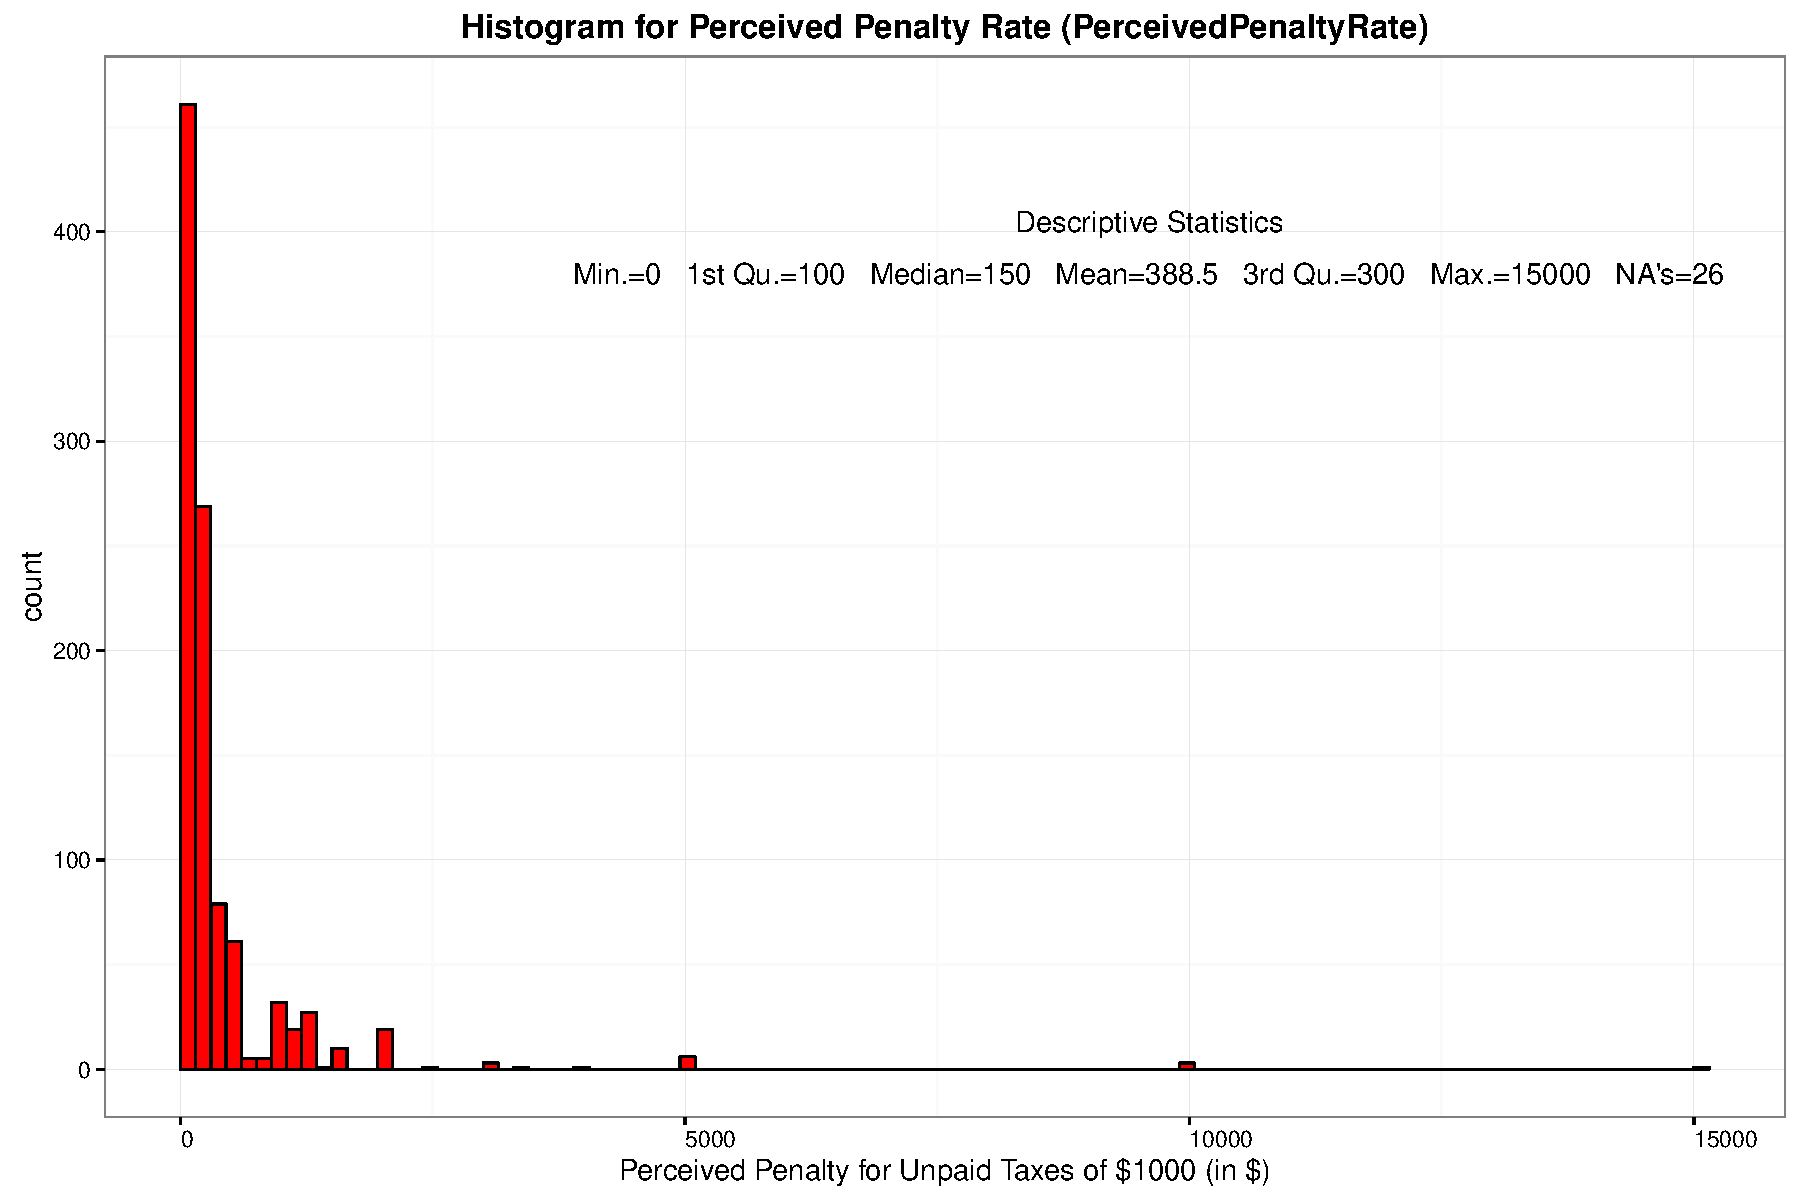
\includegraphics[width=5in]{HistPerceivedPenaltyRate.pdf} 
   \label{Fig:PerceivedPenaltyRate}
\caption{}
\end{figure}

\clearpage 
\pagenumbering{arabic}
\renewcommand{\thepage} {Ref--\arabic{page}}

%\bibliographystyle{unsrtnat}
\bibliographystyle{apalike}
\bibliography{tax_evasion}

\end{document}


%Microdata: Survey
%Macrodata: Tax compliance used for calibration. 
